
\chapter{System architecture and specifications}


% În acest capitol vom începe prin a descrie care sunt obiectivele sistemului prezentat în această lucrare. 
% Urmand sa detaliam pasi de dezvoltare a celor doua prototipuri. Totodată vom pune în evidența care sunt capabilitățile aplicaților. Iar la final vom dezbate eventuale extinderi si rezultate obtinute.


In this chapter we will begin by describing the objectives of the system presented in this paper. 
We will provide information on the development of the two prototypes. 
At the same time, we will highlight the capabilities of the application. Finally, we will discuss possible extensions and results.

\section{Goals}

\par Our motivation is to help patients who need physiotherapy to see a progress and to encourage them to be 
constant during their treatment. We want to support patients motivation in continuing to build new and 
 healthy behaviours. But also helping Physiotherapist in evaluation of patient.

% Obiectivul principal este cel de a urmari pacientul in timp ce isi face exerciti 
% ca sa ajutam kinetoterapeutul in evaluare pacientului si sa motivam pacientul prin raportarea progresului. 
The primary objective is to track the patient while he doing exercise to help 
the physical therapist in evaluation of patient and to motivate the patient by reporting progress.

% In acest sens am implementat peste algoritmul de estimare a posturi cele doua abordari detaliate in introducerea lucrari,cel care caulculeaza rang of motion si calcularea distantelor pentru afisarea progresului pacientului.

In this case, we implemented the pose estimation algorithm, 
the two approaches detailed in the introduction of the papers, 
the one that calculate Range of Motion  and the calculation of the distances for display the progress of the patient

% Dar pentru realizarea acestui obiectiv avem nevoie ca algoritmul de estimare a posturi sa aiba o performanta de minim 30 fps
% care sa poata rula atata in browser cat si pe dispozitive mobile.
But to achieve this goal, 
we need the pose estimation algorithm to have a minimum of 30 fps that can run both in the browser and on mobile devices.

% In continuare ne vom exact pe rularea algoritmilor de detectare a posturi
%  in timp real pe imagini de la camera video la o performanta de minim 30 de framuri pe secunde.
%  Dar si pe gasirea arhitecturile de retele neuronale de convolutie care sa permita acest lucru.
Next we will accurately run real-time pose estimation algorithms on the video camera at a performance of at least 30 frames per second.
  But also finding convolution neural network architectures to allow this.

%  Nu dorim folosirea unui server care sa primesca acest stream-urilor de imagini si sa aplice algoritmi de detectie
%   datorita calculelor foarte costisitoare ca timp si volumului mare de date care trebuie procesate.
We do not want to use a server that are to receive the streams of images 
and apply detection algorithms due to calculations costly in time and volume of data to be processed.

% Varianta cu servar a fost implementat dar mare problema a fost delay de 3-4 sec 
%   astfel obiectivul nostrul minim 30 de framuri pe secunda nu putea fi realizabil.
The server variant was implemented but the big problem 
was a delay of 3-4 sec so our goal of at least 30 frames per second could not be achieved.


% Pentru a obtine performance maxime a algoritmilor este necesara rularea lor pe placa grafica a aplicatie client.
To achieve maximum performance of the algorithms, 
it is necessary to run them on the GPU of the client application. 

%  Noi am propus implementare a doua prototipuri , o aplicatie web si una mobile. 
 We proposed the implementation of two prototypes, a web application and a mobile application.
%  Fiecare aplicatie implementeaza o abordarea diferite care foloseste o arhitectura defirita de retea neuronala de convolutie
Each application implements a different approach that uses a different type of architecture from convolution neural network.


%  Aplicatia mobile va calcula distantele facute de mainile si picioarele pacientului in timpul unui exercitiu 
%  astfel generand raporte cu performanta de la o zi la alta pentru a imbunatati motivarea pacientului.

The mobile app will calculate the distance traveled by the hands and legs during an exercise that the 
patient will perform, generating reports with day-to-day performance to improve motivation of the patient.



%  Aplicatie web calculeaza Range of Motion pentru a ajuta pacientul sa faca corect exercitile, astfel vom numara numarul de repatari corecte pe baza unghiurilor care le optine pacientul in timpul exercitiului
The web application will calculate a range of motion to help the patient perform the correct exercises, so we will count the correct number of repetitions of an exercise based on the angles that help the patient during the exercise.

\section{Mobile - Application development}

In acest capitol vom vorbi implementarea aplicatie mobile. Prezentand principale aspecte care au dus la rezultatele obtinute.


\subsection{Specification of the problem}
 
\par This application is designed to help everyone who need physiotherapy treatment to stay motivated,
 reach their goals, and create habits that are healthy and helpful for a long term. 
 In this case we have a solution by creating a app which will be a useful tool for patients who needs help 
 to reach their goals by automated tracking of distances.
 
 
\subsection{Analysis and design}
Aplicația care vine să demonstreze capabilitățile algoritmului de urmărire posturi și de determinare a poziției membrelor, este de tip client-server.

Clientul este o aplicatie mobile, find compatibila atata cu systemul Android cat si cu IOS. 
Vom oferi posibilitatea utilizari systemului si fara conexiune la internet, datorari utilizari librarie firebase.

Serverul este compos din mai multe servici oferit de google cloud, sub denumirea Firebase. Serviciul Firestore faciliteaza operatile CRUD pe resurse precum programul de exerciti. Cloud Function ofera  executia de function custom pentru a implementa logica de bussnise. Datele vor fi stocate intr-o baza de date NOSQL de catre serviciul Firestore. Comunicare dintre aplicatie client si servar se face prin protocolul Http, 

 Figura \ref{fig:uml-client-server} prezintă o diagramă în care se pot vedea relațiile dintre client și servicile firebase.
 
 \begin{figure}[htbp]
	\centerline{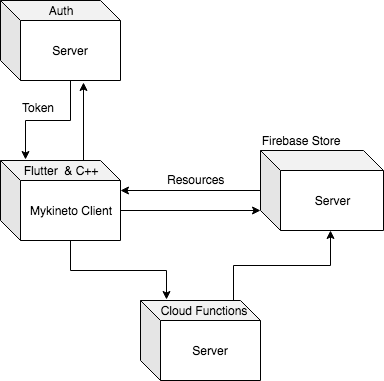
\includegraphics[scale=0.7]{fig/client-server.png}}  
	\caption{Diagrama de implementare}
	\label{fig:uml-client-server}
\end{figure}

Scopul este dea a motiva pacientul prin raporte zilnice cu activitatea lui.
In acest sens se va rula in timp real algoritmi de pose estimation pe imaginile reciptionate 
de la camera telefonului mobil si vom salva datele generate in firebase.
In Figura \ref{fig:uml-mobile} putem observa modul in care se salveaza datele obtinute de la algoritmul de pose estimation.
Astfel de fiecare daca cand incepem sa facem un exercitiu se creata o noua sessiune unde ajung sa fie salvate toate miscarile care algoritmul le-a detectat in timp ce facem exercitul.
 \begin{figure}[htbp]
	\centerline{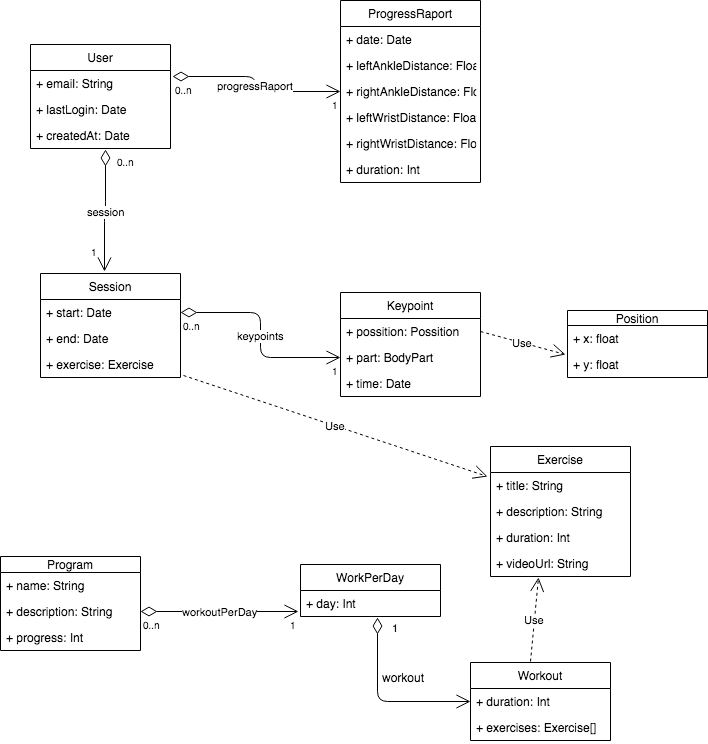
\includegraphics[scale=0.6]{fig/uml-mobile.png}}  
	\caption{Diagrama de clase}
	\label{fig:uml-mobile}
\end{figure}

Pentru detectarea vom folosi o reata neuronala de convolutie cu o arhitectura specializata in estimarea posturilor.
Arhitectura retelei este descrisa in articolul "Convolutional pose machine" \cite{DBLP:journals/corr/WeiRKS16}.
Acesta retea a fost implementat in python folosind libraria tensorflow. Dupa antrenarea ei am obtinut un model 
care a fost convertit in unul optimizat pentru a rula pe dispozitive mobile, numit tensorflow lite.
Dupa testarea lui sa constat ca performantele sunt slabe datorita rulari lui pe CPU.

Dupa un research am descoperit o librarie care stie sa convertesca modelul tensorflow lite intr-un model capabil sa 
folosesca placa grafica. Acesta librarie se numeste Mobile AI Compute Engine (MACE)  care a fost dezvoltata de cei de la XiaoMi. Pentru a putea folosi MACE a trebui sa integram o legatura dintre android si C++, deoarece macea este scris in C++ folosind Android NDK.
In urma integrari sa obtinut performate mult mai bune, ajungand la 30-40 de framuri pe secunda.
Obinund o rularea a modelului in 17 ms.

Mai sus am descris cum se salveaza sesiuni in timp ce utilizatorul face exerciti.
Pe baza acestor sesiuni se vor genera raporte. Astfel se foloseste un cloud function care ia toate sesiunile din ziua curenta si genereaza un ProgressReport, conform diagramei din Figura \ref{fig:uml-mobile}.
In urmatorul capitol vom da mai multe detali legate de implementarea aplicatie.

\subsection{Implementation}
Pentru implementarea aplicatie sa folosit Flutter.
Flutter este un framework facut de cei de la google, este scris in limbajul de programare Dart. Permitea rularea aplicatilor pe mobile, desktop, web si dispozitive IoT. Acesta este orientat pe componente oferind o reutilizarea a codului crescuta.

Daca am face o compoaratie in Flutter si React Native putem observa ca din punct de vedere arhitectural ambele implementeaza concepte asemanatoare, cum ar fi componentele, provider consumer, arhitectura de Flux.
Dar mare diferenta consta in implementarea interna total diferita.
React native foloseste componente native de android, prin folosirea unui cancal de comunicare pentru componenta din javascript si cea native.
Flutter a renuntat la acesta idee , nu mai folosind componente native, a recurs la desenarea acestora direct prin
api internat care defapt il folosesc si componentele native pentru a fi desenate pe UI.

%  \begin{figure}[htbp]
% 	\centerline{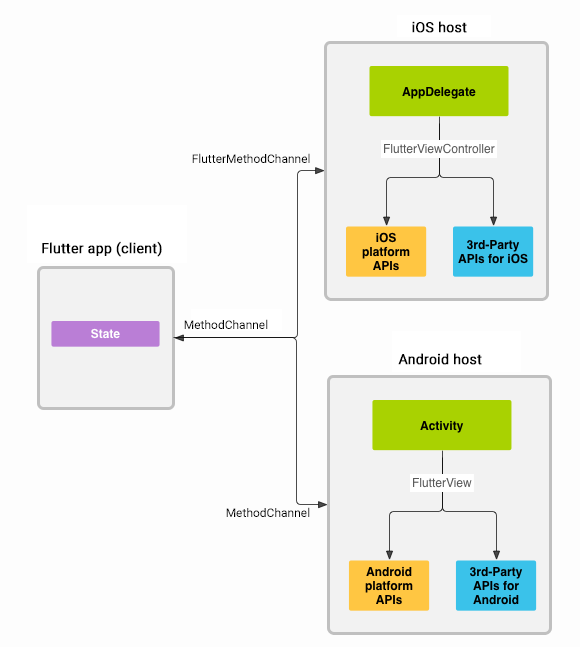
\includegraphics[scale=0.7]{fig/PlatformChannels.png}}  
% 	\caption{Architectural - Platform channels \cite{flutter}}
% 	\label{fig:flutter-plaform-channels}
% \end{figure}

Ca sa integram partea de pose estimation a fost nevoie de a deschide un activity din android folosindune de arhitectura Flutter care permite comunicare dintre codul scris in dart cu cel scris in java. In Figura  \ref{fig:flutter-plaform-channels} putem observa acesta arhitectura.

Pentru a obtine performante mari ale algoritmului de estimare a posturi am folosit MACE care vine cu o metoda de a converti modelul din tensorflow intr-un model care poate rula in C++ folosind placa grafica a telefonului.
Ca sa desenam sckeletul obtinut de algoritm vom folosi opencv. 

Ca sa generam raporte vom rula un cloud function care va prea datele de la fiecare sesiune de exerciti si le va procesa pentru a obtine distantele parcurse.
Acesta distanta va fi calculata cu ajutorul formulei matematice a distantei euclidiane.
AStfel vom parcurse tot cate doua estimari de poziti si vom face disnta din ele. Algoritmul va exclude distantele foarte mici pentru a scadea erroare de calcul.


\subsection{User manual}



Aplicația este disponibilă momentan doar pentru
sistemele de operare android, chiar dacă varianta finală este
cross-platform, fiind disponibilă și în varianta iOS, din cauza
lipsei unui telefon cu sistem de operare iOS, nu putem garant
buna funcționare a aplicatie. O puțeti descărca pe Google Play
la acest link:https://play.google.com/store/apps/details?id=com.mykineto
sau o puteți să folosiți apk de pe CD atașat lucrări.

\begin{figure}[!htb]
  \centering
  \subfloat[Login]{
    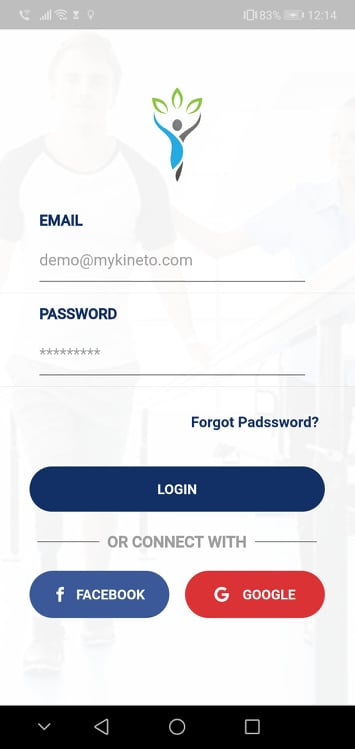
\includegraphics[width=0.3\textwidth,height=0.55\textwidth]{fig/screen-login.jpg}\label{fig:screen-login}}
  \hfill
  \subfloat[Rehab program]{
    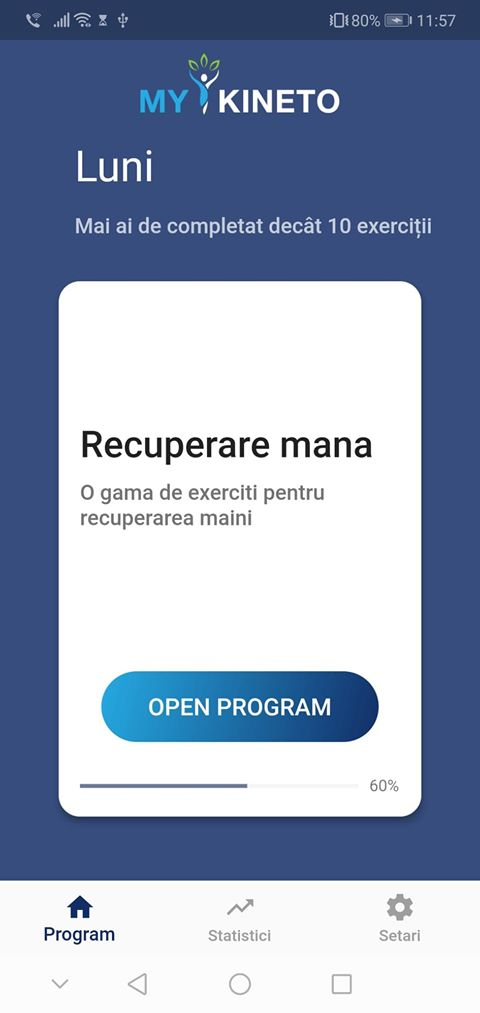
\includegraphics[width=0.3\textwidth,height=0.55\textwidth]{fig/screen-program.jpg}\label{fig:screen-program}}
    
    \caption{Screen with login and rehab program}
\end{figure}

Pentru rularea aplicației aveți nevoie de un telefon cu
sistemul de operate android la versiune minimă 4.3.
După instalarea apăsați pe aplicați pentru a se deschide.
O să apară fereastra din Figura \ref{fig:screen-login}.
Utilizatorul se va autentifica in aplicatie, dupa care va vedea o lista de cu programe de recuperare.
Va intra pe un program de recuperare unde va isi va alege ziua in care va efectua exercitul.


\begin{figure}[!htb]
  \centering
  \subfloat[Workout]{
    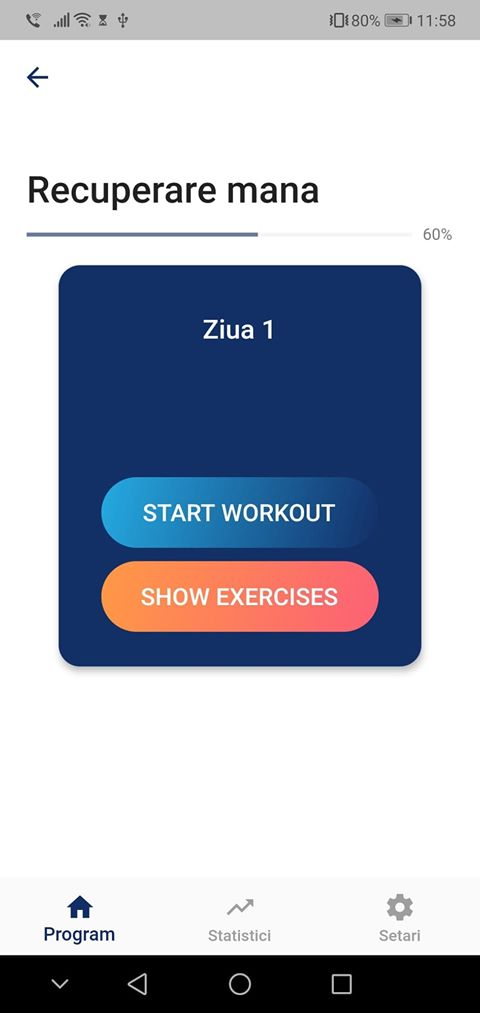
\includegraphics[width=0.3\textwidth,height=0.55\textwidth]{fig/screen-workout.jpg}\label{fig:screen-workout}}
  \hfill
  \subfloat[Exercise]{
    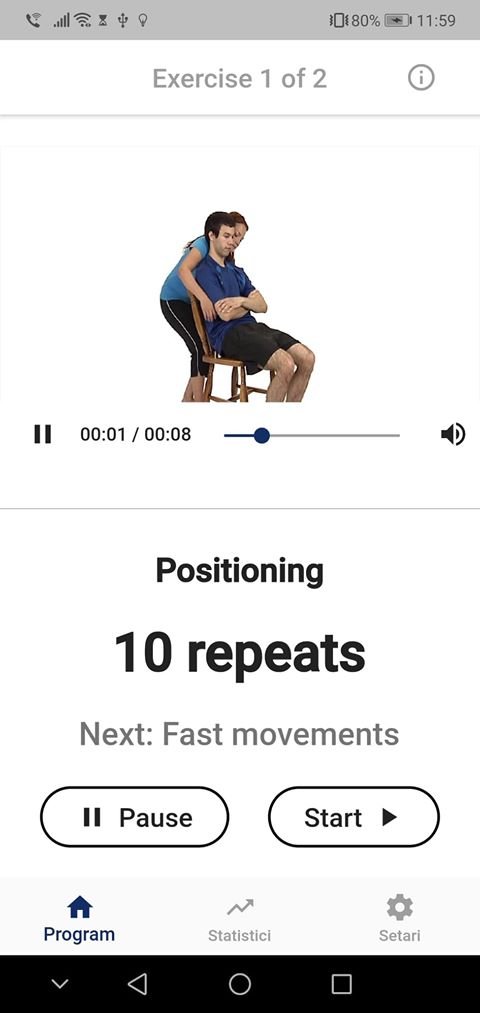
\includegraphics[width=0.3\textwidth,height=0.55\textwidth]{fig/screen-exercise.jpg}\label{fig:screen-exercise}}
    
    \caption{Screen with workout and exercise}
\end{figure}

Dupa alegerea zilei, utilizatorul va incepe sa faca exercitile in fata camerai telefonului.
Aplicatia va monitoriza si salva miscarile facute de utilizator in timpul fiecarui exercitiu.

\begin{figure}[!htb]
  \centering
  \subfloat[Pose Estimation]{
    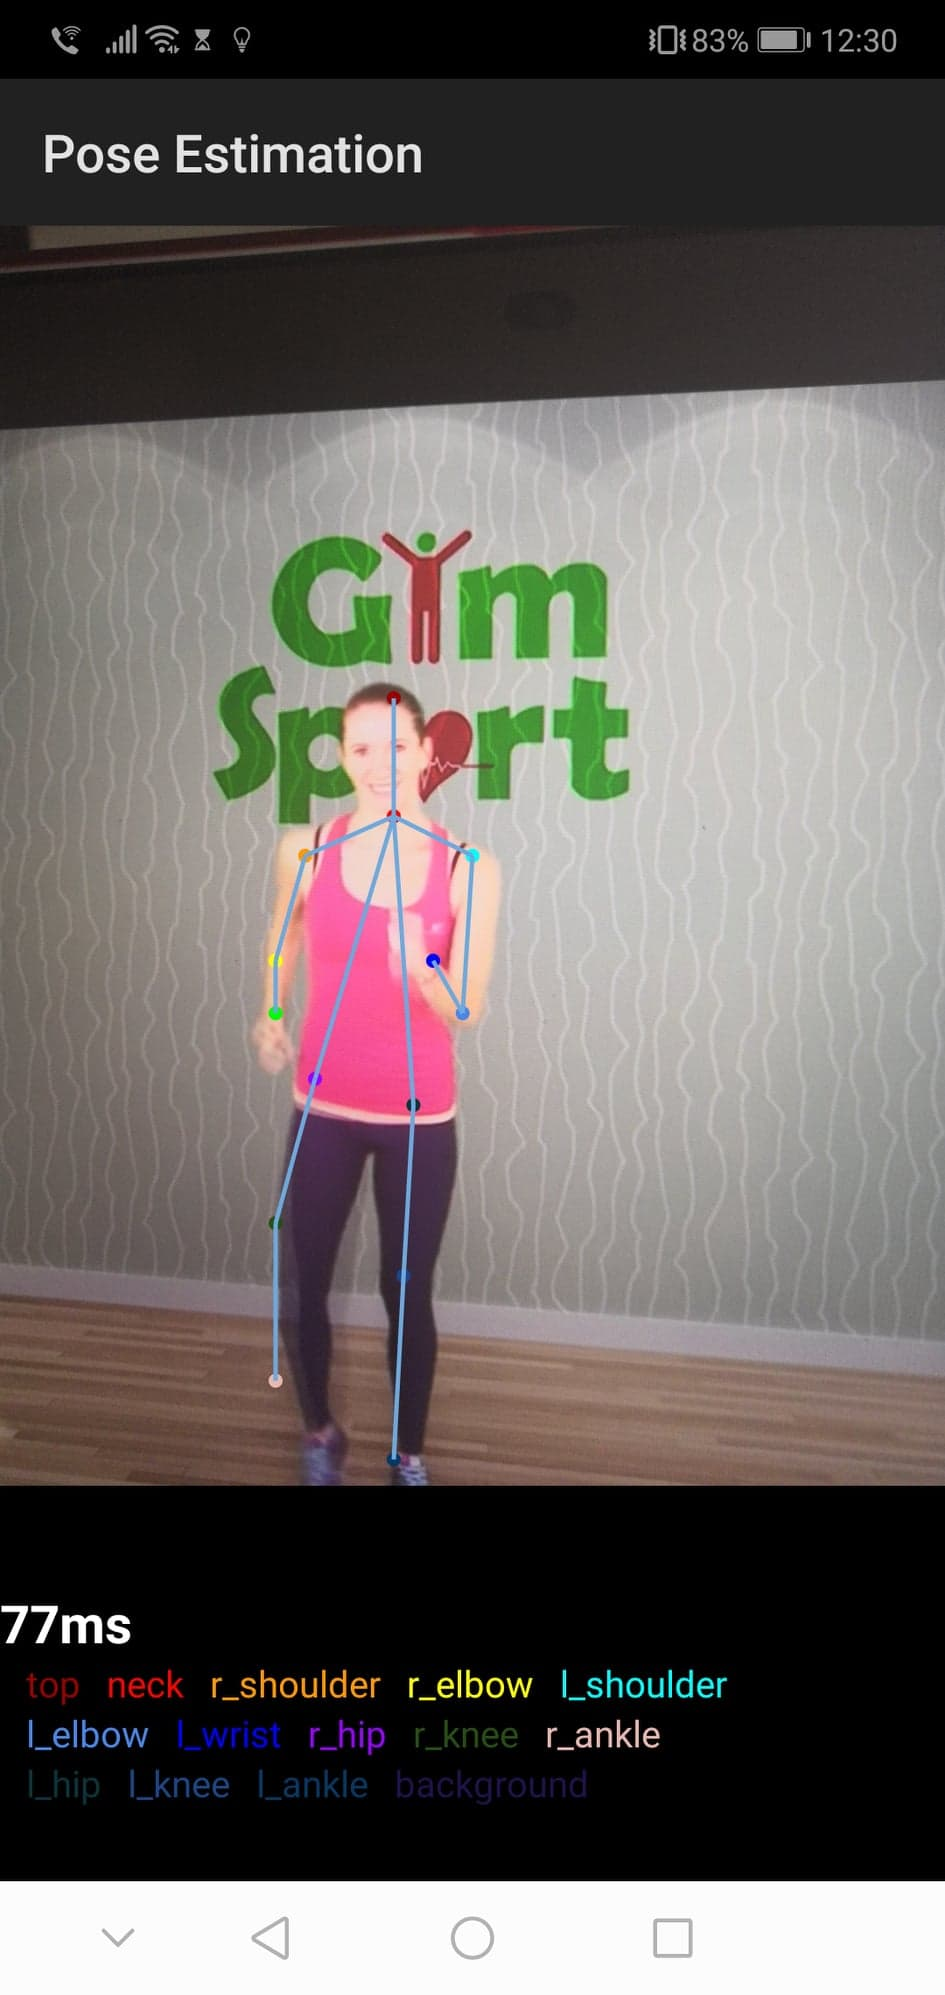
\includegraphics[width=0.3\textwidth,height=0.55\textwidth]{fig/screen-pose.jpg}\label{fig:screen-pose}}
  \hfill
  \subfloat[Statistics]{
    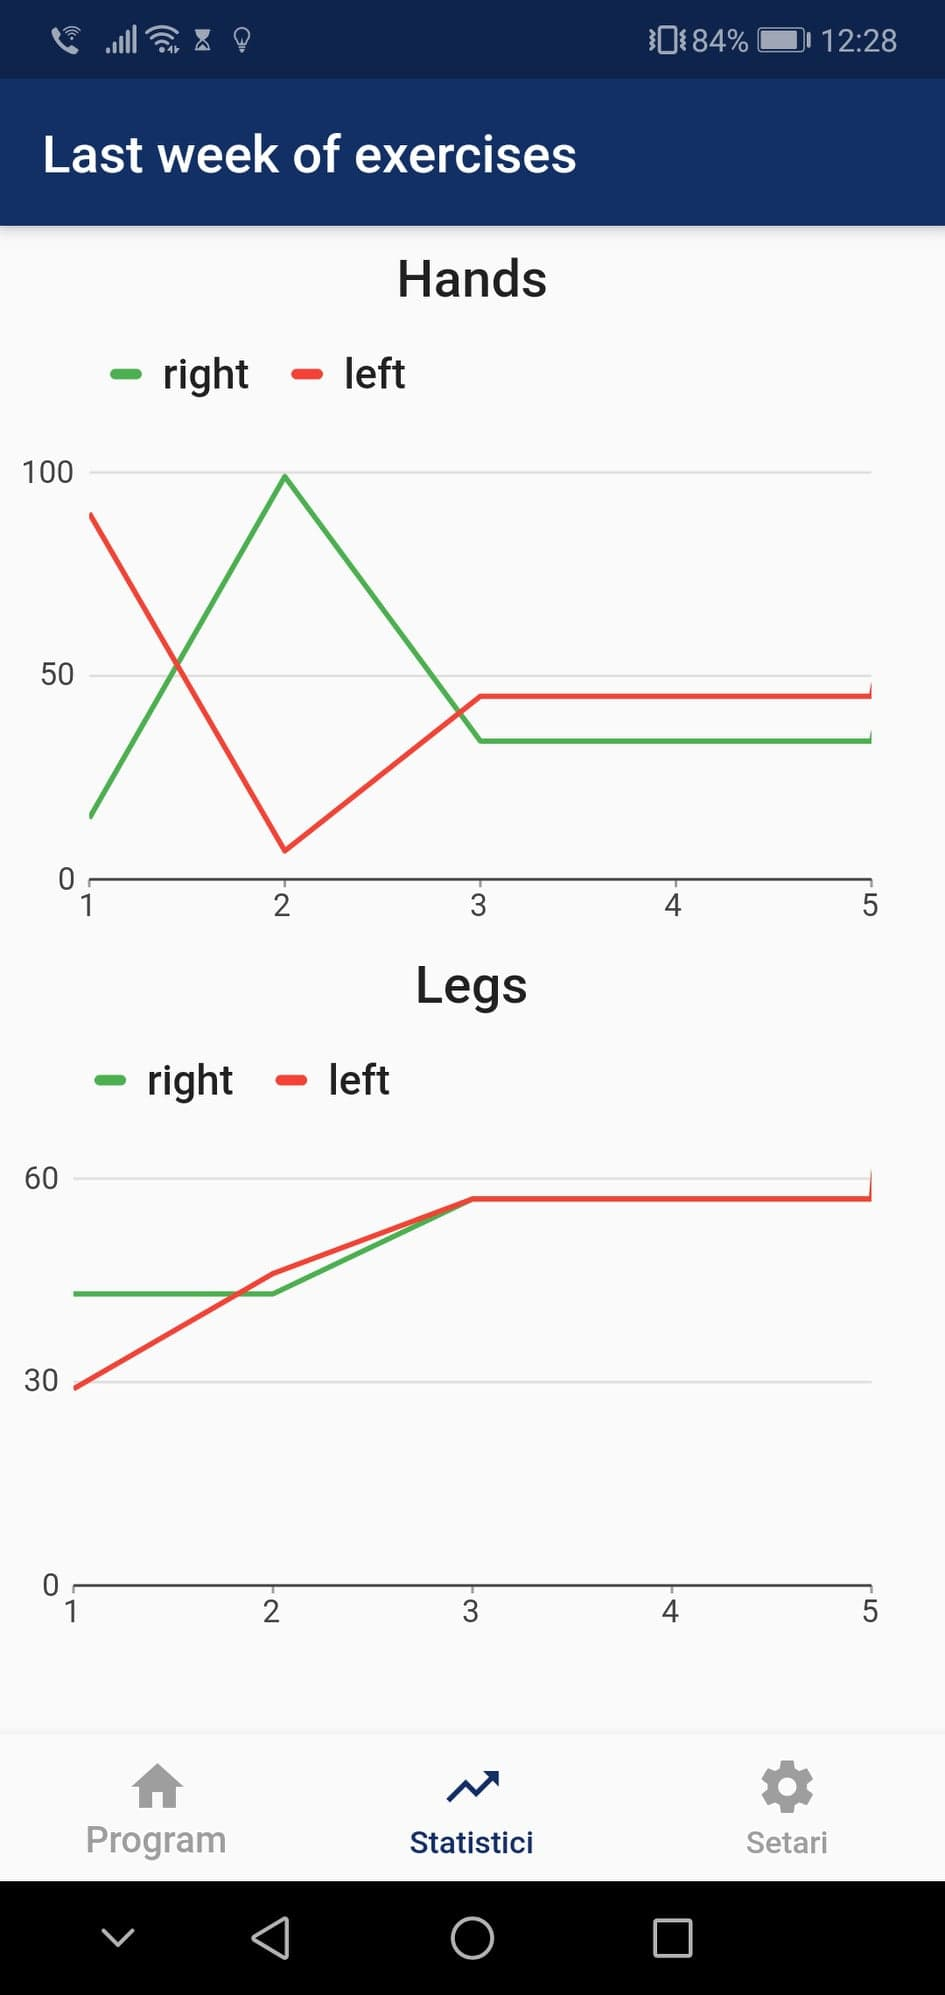
\includegraphics[width=0.3\textwidth,height=0.55\textwidth]{fig/screen-progress.jpg}\label{fig:screen-progress}}
    
    \caption{Screen with pose estimation and progress}
\end{figure}
Utilizatorul va putea viziualiza statisticile pe zile a progresului facut de in el timpul antrenamentului. 

\section{Web - Application development}

In acest capitol vom descrie modul in care a fost dezvoltat aplicatia suprinzand principale algoritmi folosinti. 
Continund cu detalile de implementare care au contribuit la acesta aplicatie.



\subsection{Specification of the problem}

Application is an interactive software destined for patients who need physiotherapy
treatments. Our application guide patient to see how they need to make their exercises in 
a correct manner by showing Range of Motion (ROM) in real time and after allowing us to 
 count the number of movements. 
 
It is based on exercices, because we think that a constant and correct number of movements could be more efficient for patients then just to present them what exercices they need to do. In this manner the application guides each patient during the all period they need to follow their treatment. 

\subsection{Analysis and design}

Aplicatia va rula in browser folosind camera web pentru a detecta in real-time postura pacientului.
Oferindune cordonatele membrelor acestuia pe baza carora vom aplica algoritmul de calculare a unghiurilor, obtinand astfel range of motion. 
In acest sens vom folosit tensorflow.js care permitea rularea in browser a algoritmului de inteligenta artificiala.
Noi vom folosi modelul PoseNet.

PoseNet este un model antrenare care are la baza o reatea neuronale de convolutie, find invatata sa clasifice partile corpului dand ca rezultat cordonatele acestora. In figura \ref{fig:uml-posenet} se poate observa o diagrama care prezinta structura deletor de iesire care le ofera PoseNet.

 \begin{figure}[htbp]
	\centerline{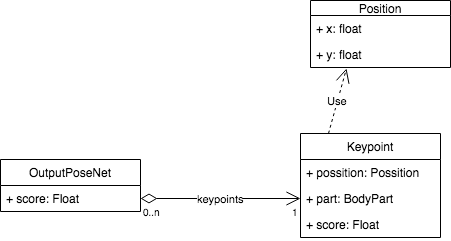
\includegraphics[scale=0.7]{fig/uml-posenet.png}}  
	\caption{PoseNet output}
	\label{fig:uml-posenet}
\end{figure}

PoseNet a fost realizat de cei de la google si foloseste o arhitectura de tip MobileNet.
MobileNet este o arhitectura optimizata pentru a rula pe dispozitive fara putere mare de calcul.
 
In articolul " Mobilenets:  Efficient  convolutional  neuralnetworks for mobile vision applications"  \cite{DBLP:journals/corr/HowardZCKWWAA17} sunt descrise principale optimizare aduse de arhitectura numit MobileNet.
Cea mai importanta optimizare de performanta a fost realizata prin introducerea unui nou tip de strat, numit Depthwise Separable Convolution. Acest strat inlocuieste convolutila standard. Si mare diferenta este ca a impartit in doi pasi separati, aplicarea filtrari si combinarea.

Pe baza keypoints obtinute de la PoseNet vom desena unghiurile dintre membrele pacientului folosind canvas.
Unghiul dintre doua drepte va fi calculat folosind formula matematica, reprezentand range of motion.

Pentru a numara numarul de exerciti corecte vom folosi un algoritm bazat pe unghiuri pentru fiecare tip de exercitiu.

De exemplu daca se fac squats atunci algoritmul va functiona pe baza de stari, astfel vom avea starile:
\begin{itemize}
    \item Inceputul exercitiului daca unghiul de la genunchi este intre 10 si 75 de grade
    \item Sfarsitul exercitiului daca unghiul de la genunchi este intre 145 si 300 de grade
\end{itemize}

Pe baza acestor doua stari, vom numara numarul de exerciti facute corect din puncte de vedere a unghiului genunchiului.

 \begin{figure}[htbp]
	\centerline{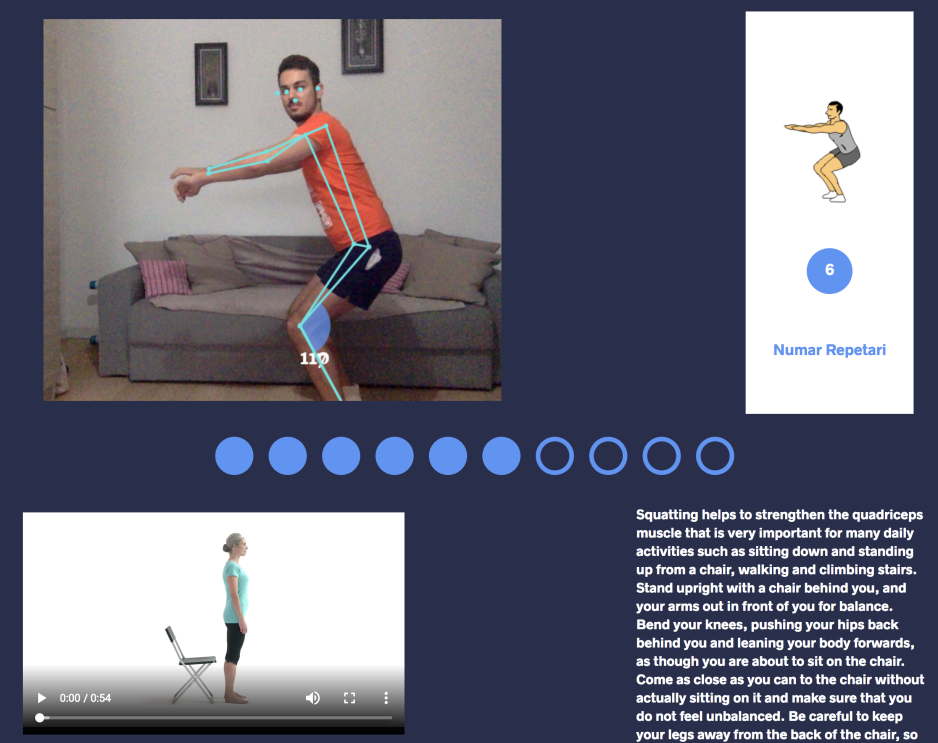
\includegraphics[scale=0.7]{fig/demo-mykineto.png}}  
	\caption{Demo MyKineto}
	\label{fig:demo-web-mykineto}
\end{figure}

In Figura \ref{fig:demo-web-mykineto} se poate vedea cum algoritmul numara numarul de repetari corecte si
afiseaza punctele detectate in timp real de algoritm folosind canvas.




\subsection{Implementation}

Pentru implementarea acestei aplicatie web sa folosit react in dezvoltarea interfetei grafice.
Iar pe partea de pose estimation am folosit tensorflow.js impreuna cu modelul PoseNet.

Ce este React? React este o bibliotecă JavaScript folosită în dezvoltarea interfețelor web.
Prima versiune a fost lansată de către facebook în Martie 2013. Față de alte platforme React vine cu
capacitatea sa de a fi declarativ, bazat pe componente și faptul că este reutilizabil \cite{fb-react}.

Biblioteca React permite crearea de componente pentru fiecare stare a aplicației, în cazul
modificări unei stări se vor randa componentele care trebuie să apară în cazul acelei stări, astfel se
crește performanța aplicației.

React folosește noua sintaxă JavaScript Extension (JSX) care este asemănătoare cu sintaxa
Hypertext Markup Language (HTML), defirența este că pe post de marcatori putem folosi
componente React \cite{jsx-react}.

O cauză a modelului declarativ bazat pe componente constă în reutilizarea codului, fiecare
componentă își încapsulează și gestionează propria stare. Se pot realiza interfețe complexe prin
asamblarea lor precum niște pazăluri. Fiecare componentă își gestionează, asta este un task dificil în
realizarea unor arhitecturi complexe.

Pentru o eficiență mai sporită, React folosește Virtual DOM, care este o abstractizare a
DOM, fiindcă operațiile asupra DOM sunt încete \cite{virtual-dom-react}.

Tensorflow.js permite rula algoritmilor de inteligenta artificala in mediul javascript.
Dupa cum stim algoritmi de inteligenta artificiala, mai ales cei aplicati pe imagini sau video au nevoie
de o putea mare de calcul.
Pentru a rezolva acesta problema, tensorflow.js ruleaza algoritmi folosind WebGL in mod automat.
Acest lucra face ca algoritmi sa ruleze pe GPU \cite{tensorflow.js}.


Pe lângă asta, pentru dezvoltarea aplicație s-a folosit typescript care este un super set tipizat a lui javascript și mediul de dezvoltare Visual Studio Code.

\section{Experimental results}

In urma implementari celor doua variante de mai sus am facute mai multe teste legate de performanta algoritmilor.
Mai exact cat de repede ruleaza algoritmul de pose estimation pe o imagine. Cu cat ruleaza mai repede cu atata optinem o performanta mai buna, targul nostru find de 30 frame per seconds.


 \begin{figure}[htbp]
	\centerline{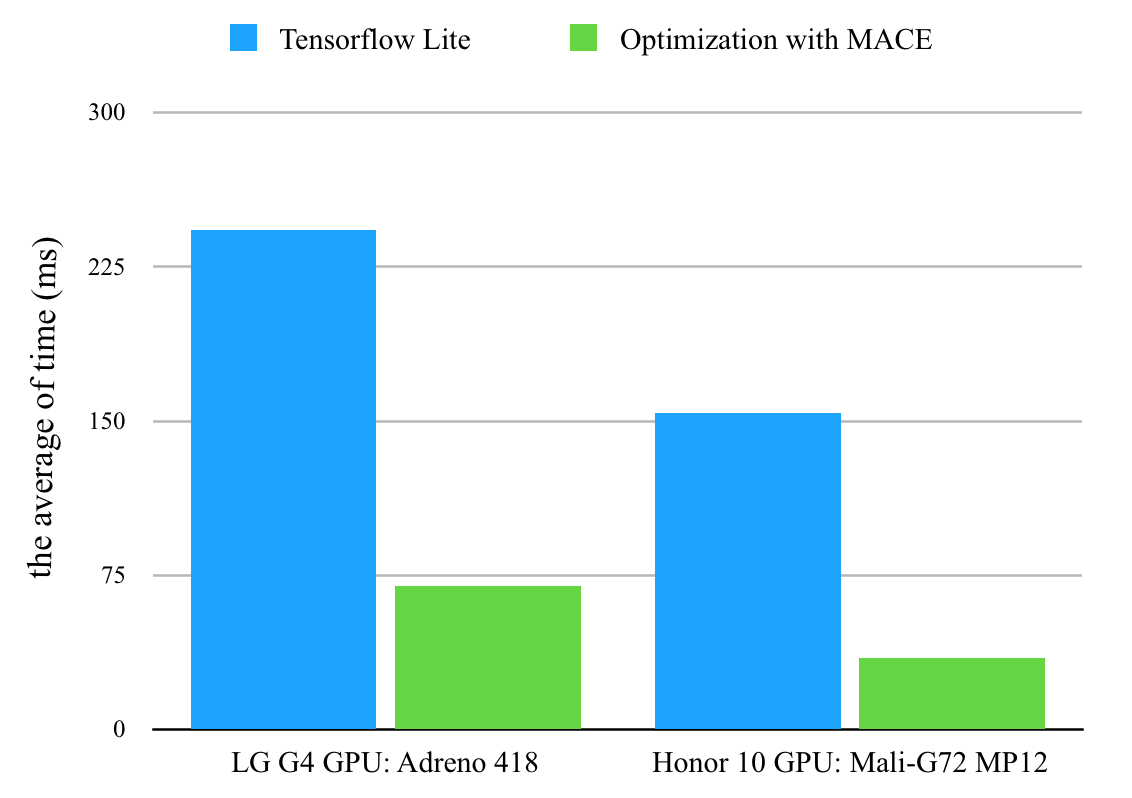
\includegraphics[scale=0.7]{fig/mobile-performace.png}}  
	\caption{The performance of the pose estimation algorithm run on two devices with optimized and non-optimized model.}
	\label{fig:mobile-perf}
\end{figure}

In Figura \ref{fig:mobile-perf} putem observa o create cu 50\% a performantei in cazul modelul optimizat pentru aplicatie mobila.

In cazul aplicatie web, lucrurile stau un pic diferit. Am incerc sa fac o comparatie intre rularea algoritmului pe client sau pe server. Se poate observa clar din figura \ref{fig:web-perf} ca varianta cu servarul se exclude doarece ori cat ar fi servarul de bun durata requestului dureaza in medie 50 ms doarece se trimit un numar mare de date.


 \begin{figure}[htbp]
	\centerline{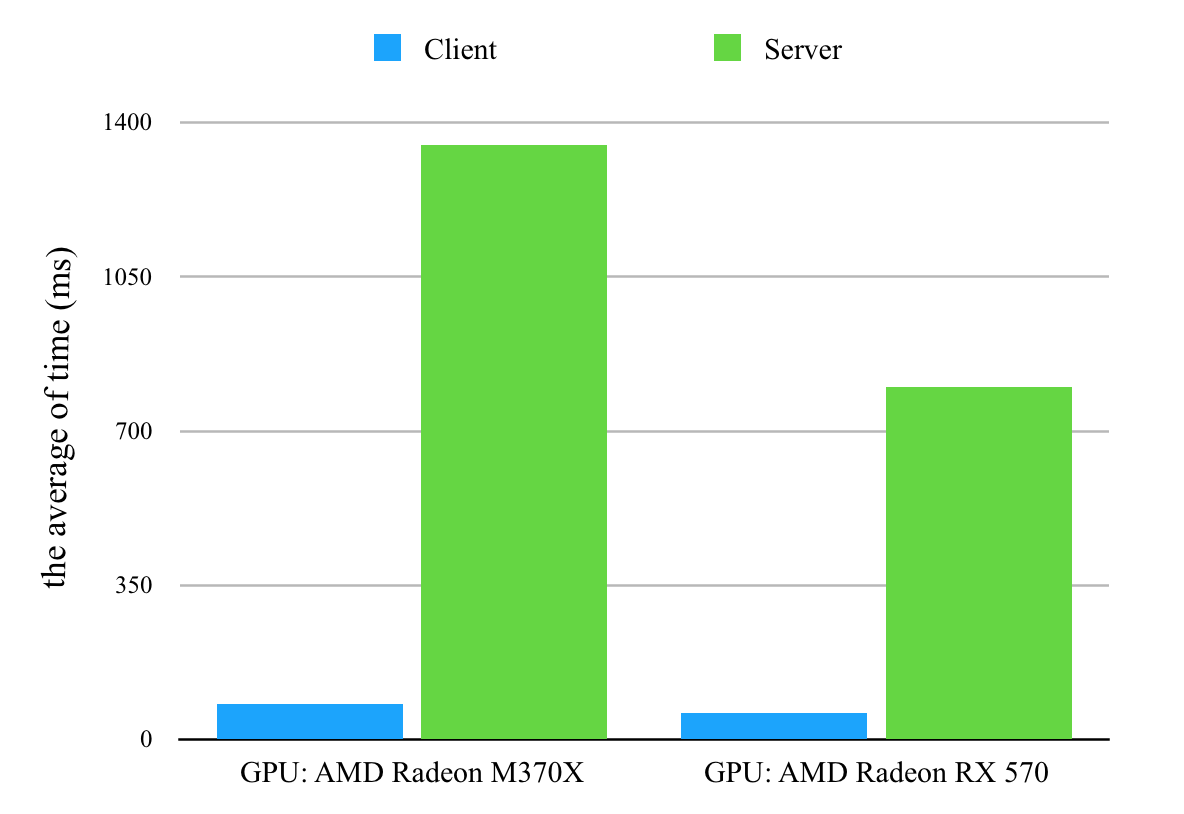
\includegraphics[scale=0.7]{fig/web-performace.png}}  
	\caption{The performance of the pose estimation algorithm run on web}
	\label{fig:web-perf}
\end{figure}

\section{Possible extensions}


